\documentclass{cheatsheet}
\usepackage{bm}
\usepackage{textcomp, mathcomp}
\usepackage{pbox}
\usepackage{amsmath, amssymb, mathtools, empheq, physics}
\usepackage{xcolor}
\usepackage{graphicx}
% for wild tikz drawings
\usepackage{tikz}
\usepackage{pgfplots}
\usepackage{mathdots}
\usepackage{yhmath}
\usepackage{cancel}
\usepackage{color}
\usepackage{siunitx}
\usepackage{array}
\usepackage{multirow}
\usepackage{amssymb}
\usepackage{gensymb}
\usepackage{tabularx}
\usepackage{extarrows}
\usepackage{booktabs}

\usetikzlibrary{fadings}
\usetikzlibrary{patterns}
\usetikzlibrary{shadows.blur}
\usetikzlibrary{shapes}

\doctitle{Analysis 2 Cheatsheet}
\author{\href{https://n.ethz.ch/\~bmicha}{Micha Bosshart} - bmicha@ethz.ch \\ \vspace*{-0.2em}}

%\def\HyperFirstAtBeginDocument#1{#1} 
\begin{document}
    \section{Funktionen}
        % !TeX root = ../../ZF_bmicha_Ana.tex
\subsection{Folgen und Reihen}
    \begin{description}
        \item[konvergent] Es existiert ein Grenzwert sonst divergent.
        \item[beschränkt] Alle Glieder in \emph{endlich breitem}, \emph{waagerechten Parallelstreifen} enthalten.
        \item[monoton wachsend] $\quad a_{n+1} \geq a_n \qquad  (\emph{strikt}:\,\, >)$
    \end{description}
    \fbox{mon. wachsend/ fallend \& beschränkt $\Rightarrow$ konvergent}
    \subsubsection{Rechenregeln für konvergente Folgen}
        Falls $\displaystyle \lim_{n\to \infty} a_n = a$ und $\displaystyle \lim_{n\to \infty} b_n = b$, gilt:
        \begin{align*}
            \lim_{n \to \infty}(a_n \pm b_n) &= a \pm b\\
            \lim_{n \to \infty}(a_n \cdot b_n) &= a \cdot b\\
            \lim_{n \to \infty}(a_n / b_n) &= a / b.
        \end{align*}
        Gilt auch für Funktionen; sofern Grenzwert existiert.
        % \vspace*{-1em}
    \subsubsection{Geometrische Reihe}
        \begin{align*}
            \sum_{n=0}^{k}a \cdot q^n &= a \cdot \frac{1 - q^{k+1}}{1-q\phantom{^{k+1}}}\\
            \sum_{n=0}^{\infty}a \cdot q^n &= \frac{a}{1-q}, \quad \textrm{falls } \abs*{q} < 1
        \end{align*}
        \vspace*{-0.5em}
    \subsubsection{Arithmetische Reihe}
        $$
            \sum_{n=1}^{\infty} \ [a_1 + (n-1) \cdot d] = \frac{n}{2} \cdot (a_1 + a_n)
        $$
    \subsubsection{häufige Reihen}
        \vspace{0em}
        \begin{itemize}
            \item $\displaystyle \sum_{n=1}^{k} n = \frac{k \cdot (k + 1)}{2} $ \hspace*{0em} $\triangleright \displaystyle \sum_{n=0}^{\infty} \frac{1}{n!} = \lim\limits_{n \rightarrow \infty} \left(1 + \frac{1}{n}\right)^n = e$
            % \item $\displaystyle \sum_{n=0}^{\infty} \frac{1}{n!} = e$
            \item $\displaystyle \sum_{n=1}^{\infty} \frac{1}{n^{\alpha}}
            \begin{cases}
                \alpha = 1 \rightarrow \text{ harm. Reihe}\\
                = \infty, \alpha \leq 1 \text{ (divergiert)}\\
                \neq \pm \infty, \alpha > 1 \text{ (konvergiert)}
            \end{cases}
            $
        \end{itemize}
        
        \subsection{Grenzwerte}
        \subsubsection{Bernoulli de L'H$\hat{\textrm{o}}$pital}
    Falls $\displaystyle \lim_{x \to a} f(x) = \lim_{x \to a} g(x) = 0$ (oder $\pm \infty$), so gilt
    $$
         \lim_{x \to a} \frac{f(x)}{g(x)} = \lim_{x \to a} \frac{f'(x)}{g'(x)}.
    $$
        \input{src/Funktionen/landau_symbole.tex}
        \input{src/Funktionen/eigenschaften.tex}
        \input{src/Funktionen/asymptoten.tex}
        \input{src/Funktionen/hyperbolische_funktionen.tex}
    \section{Komplexe Zahlen}
        % !TeX root = ../../ZF_bmicha_Ana.tex
\tikzset{
    pattern size/.store in=\mcSize, 
    pattern size = 5pt,
    pattern thickness/.store in=\mcThickness, 
    pattern thickness = 0.3pt,
    pattern radius/.store in=\mcRadius, 
    pattern radius = 1pt}
    \makeatletter
    \pgfutil@ifundefined{pgf@pattern@name@_9395wxxuh}{
    \pgfdeclarepatternformonly[\mcThickness,\mcSize]{_9395wxxuh}
    {\pgfqpoint{-\mcThickness}{-\mcThickness}}
    {\pgfpoint{\mcSize}{\mcSize}}
    {\pgfpoint{\mcSize}{\mcSize}}
    {
    \pgfsetcolor{\tikz@pattern@color}
    \pgfsetlinewidth{\mcThickness}
    \pgfpathmoveto{\pgfpointorigin}
    \pgfpathlineto{\pgfpoint{0}{\mcSize}}
    \pgfusepath{stroke}
}}
\makeatother
% Pattern Info
\tikzset{
    pattern size/.store in=\mcSize, 
    pattern size = 5pt,
    pattern thickness/.store in=\mcThickness, 
    pattern thickness = 0.3pt,
    pattern radius/.store in=\mcRadius, 
    pattern radius = 1pt}
    \makeatletter
    \pgfutil@ifundefined{pgf@pattern@name@_r1aowurqw}{
    \pgfdeclarepatternformonly[\mcThickness,\mcSize]{_r1aowurqw}
    {\pgfqpoint{-\mcThickness}{-\mcThickness}}
    {\pgfpoint{\mcSize}{\mcSize}}
    {\pgfpoint{\mcSize}{\mcSize}}
    {
    \pgfsetcolor{\tikz@pattern@color}
    \pgfsetlinewidth{\mcThickness}
    \pgfpathmoveto{\pgfpointorigin}
    \pgfpathlineto{\pgfpoint{0}{\mcSize}}
    \pgfusepath{stroke}
}}
\makeatother
\tikzset{every picture/.style={line width=0.75pt}} %set default line width to 0.75pt        

\begin{center} 
    \begin{tikzpicture}[x=0.75pt,y=0.75pt,yscale=-1,xscale=1]
        %uncomment if require: \path (0,209); %set diagram left start at 0, and has height of 209
        \draw    (58.6,169.3) -- (171.85,71.95) ;
        \draw [shift={(173.36,70.65)}, rotate = 139.32] [color={rgb, 255:red, 0; green, 0; blue, 0 }  ][line width=0.75]    (10.93,-3.29) .. controls (6.95,-1.4) and (3.31,-0.3) .. (0,0) .. controls (3.31,0.3) and (6.95,1.4) .. (10.93,3.29)   ;
        \draw  (42,169.3) -- (208,169.3)(58.6,28) -- (58.6,185) (201,164.3) -- (208,169.3) -- (201,174.3) (53.6,35) -- (58.6,28) -- (63.6,35)  ;
        \draw  [draw opacity=0] (83.87,147.15) .. controls (85.33,148.6) and (86.59,150.28) .. (87.58,152.18) .. controls (90.53,157.77) and (90.52,163.98) .. (88.13,169.06) -- (70.36,160.23) -- cycle ; \draw   (83.87,147.15) .. controls (85.33,148.6) and (86.59,150.28) .. (87.58,152.18) .. controls (90.53,157.77) and (90.52,163.98) .. (88.13,169.06) ;  
        \draw [pattern=_9395wxxuh,pattern size=6pt,pattern thickness=0.75pt,pattern radius=0pt, pattern color={rgb, 255:red, 0; green, 0; blue, 0}] [dash pattern={on 0.84pt off 2.51pt}]  (173.36,70.65) -- (173.49,169.18) ;
        \draw [pattern=_r1aowurqw,pattern size=6pt,pattern thickness=0.75pt,pattern radius=0pt, pattern color={rgb, 255:red, 0; green, 0; blue, 0}] [dash pattern={on 0.84pt off 2.51pt}]  (58.36,70.65) -- (173.36,70.65) ;
    
        % Text Node
        \draw (196,174) node [anchor=north west][inner sep=0.75pt]  [font=\footnotesize] [align=left] {Re(z)};
        % Text Node
        \draw (25,26) node [anchor=north west][inner sep=0.75pt]  [font=\footnotesize] [align=left] {Im(z)};
        % Text Node
        \draw (152,50) node [anchor=north west][inner sep=0.75pt]  [font=\footnotesize]  {$z\in\mathbb{C}$};
        % Text Node
        \draw (74.22,128.61) node [anchor=north west][inner sep=0.75pt]  [font=\footnotesize,rotate=-319.68]  {$r=|z|$};
        % Text Node
        \draw (93,150) node [anchor=north west][inner sep=0.75pt]  [font=\footnotesize]  {$\varphi=\text{arg}(z)$};
        % Text Node
        \draw (169,172) node [anchor=north west][inner sep=0.75pt]  [font=\footnotesize]  {$a$};
        % Text Node
        \draw (48,65) node [anchor=north west][inner sep=0.75pt]  [font=\footnotesize]  {$b$};
    \end{tikzpicture}
\end{center}

\vspace*{0.5em}
\mathbox{
    z = \underbrace{a + ib}_{\textrm{kartesisch}} = \underbrace{r \cos(\varphi) + i r\sin(\varphi)}_{\textrm{Polarform}} =  \underbrace{r \cdot e^{i \varphi}}_{\textrm{Euler}}
}

        \input{src/Komplexe_Zahlen/nullstellen-reeller-Polynome.tex}
        \input{src/Komplexe_Zahlen/konjugierte.tex}
    \section{Potenzreihen}
        % !TeX root = ../../ZF_bmicha_Ana.tex
Potenzreihe der Funktion $f(x)$ um den Punkt $x_o$:
\mathbox{
    f(x) = \sum_{n=0}^{\infty} a_n \cdot (x-x_o)^n
}
\begin{itemize}
    \item Höchstens eine Potenzreihe von $f$ um $x_o$ existiert.
    \item Konvergiert für $\abs*{x-x_o} < r$
\end{itemize}
\mathbox{
    \frac{1}{1 - \fcolorbox{green}{white}{x}} = \sum\limits_{n = 0}^{\infty} \fcolorbox{green}{white}{x}^k
}
        \input{src/Potenzreihen/konvergenzradius.tex}
        % !TeX root = ../../ZF_bmicha_Ana.tex
\subsection{Taylorreihen}
    Taylorentwicklung von $f(x)$ um $x_o$:
    \mathbox{
        f(x) = \sum_{n=0}^\infty \frac{f^{(n)}(x_o)}{n!} (x-x_o)^n
    }
    \begin{itemize}
    \item ungerade Fkt $\Leftrightarrow$ ungerade Indizes: $a_1x + a_3x^3 + \dots$
    \item gerade Fkt $\Leftrightarrow$ gerade Indizes: $a_0 + a_2x^2 + \dots$
    \end{itemize}

        \newpage
    \section{Trigonometrie}
        \subsection{Werte Tabelle}
    \begin{center}
        \includegraphics[width=0.7\linewidth]{src/Trigonometrie/trigo_tabelle.pdf}
    \end{center}
        % \input{src/Trigonometrie/einheitskreis.tex}
        \subsection{Rechenregeln}
\vspace*{-1em}
    \begin{align*}
        1 =& \; sin(x)^2 + cos(x)^2\\
        \sin(\alpha \pm \beta) =& \; \sin \alpha \cos \beta \pm \cos \alpha \sin \beta\\
        \sin(2 \alpha) =& \; 2 \sin \alpha cos \alpha\\
        \sin(3 \alpha) =& \; 3 \sin \alpha - 4 sin^3 \alpha\\
        \sin^2 \frac{\alpha}{2} =& \; \frac{1 - \cos \alpha}{2}\\
        \cos(\alpha \pm \beta) =& \; \cos \alpha \cos \beta \mp \sin \alpha \sin \beta\\
        \cos(2 \alpha) =& \; \cos^2 \alpha - \sin^2 \alpha\\
        =& \; 2 \cos^2 \alpha - 1 = 1 - 2 \sin^2 \alpha\\
        \cos(3 \alpha) =& \; 4 \cos^3 \alpha - 3 \cos \alpha\\
        cos^2 \frac{\alpha}{2} =& \; \frac{1 + cos \alpha}{2}\\
        \frac{a}{sin(\alpha)} =& \; \frac{b}{sin(\beta)} = \frac{c}{sin(\gamma)}\\
        a^2 =& \; b^2 + c^2 - 2bc \cdot cos(\alpha)
    \end{align*}


        \subsection{Funktionsmodifikation}
\vspace*{-1em}
    \begin{align*}
        \text{Frequenz} \; f: t \rightarrow& \; \sin(\frac{2 \pi}{T} t)\\
        \text{Amplitude} \; f: t \rightarrow& \; A \cdot \sin(t)\\
        \text{Winkelgeschwindigkeit} \; \omega =& \; \frac{2 \pi}{T} \left[\frac{1}{s}\right]
    \end{align*}
    \section{Mehrdimensionale Fkt. - Diff. Rechnung}
        \input{src/Mehrdimensionale-Funktionen_Differentialrechnung/fehlerrechnung.tex}
        \input{src/Mehrdimensionale-Funktionen_Differentialrechnung/niveaulinien-flaechen.tex}
        % !TeX root = ../../ZF_bmicha_Ana.tex
\subsection{Gradient}
    $$
        \grad(f(x,y,z)) = \begin{pmatrix}
            f_x \\ f_y \\ f_z
        \end{pmatrix}
    $$
    \begin{itemize}
        \item Steht senkrecht auf Niveauflächen/ -linien.
        \item Zeigt in Richtung des grössten Anstiegs der Funktionswerte.
    \end{itemize}
    \subsubsection{2D - $f(x,y)$}
        \includegraphics[width=\linewidth]{src/Mehrdimensionale-Funktionen_Differentialrechnung/grad_2D.pdf}
    \subsubsection{3D - $f(x,y,z)$}
        \begin{center}
            \includegraphics[width=0.8\linewidth]{src/Mehrdimensionale-Funktionen_Differentialrechnung/grad_3D.pdf}
        \end{center}
        \input{src/Mehrdimensionale-Funktionen_Differentialrechnung/richtungsableitung.tex}
        % !TeX root = ../../ZF_bmicha_Ana.tex
\subsection{Tangentialebenen}
    \subsubsection{Linearisierungsformel}
        \vspace{0.5em}
        \mathbox{
            z = f(x_o,y_o) + f_x(x_o,y_o) (x\!-\!x_o) + f_y(x_o,y_o)(y\!-\!y_o)
        }
        \mathbox{
            0 = f_x(x_o,y_o,z_o)(x\!-\!x_o) + f_y(x_o,y_o,z_o)(y\!-\!y_o) + \dots
        }
    \subsubsection{Gradient}
        \begin{itemize}
            \item $f(x,y,z) = C$ ist eine Niveaufläche
            \item $\grad(f)$ steht senkrecht auf Niveauflächen. ($\to \nvec$ )
            \item Ebene mit Normalenvektor $\nvec = (A,B,C)^T$:
            $$
                Ax + By + Cz = D
            $$
        \end{itemize}
        % !TeX root = ../../ZF_bmicha_Ana.tex
\subsection{Extremalstellen von \texorpdfstring{$f(x,y)$}{f(x,y)}}
    \vspace{0.25em}
    \begin{enumerate}
        \item Inneres untersuchen $\to$ $\textrm{grad}f \overset{!}{=} 0$
        \item Rand untersuchen
        \begin{itemize}
            \item Lagrange Multiplikatoren
            \begin{enumerate}
                \item $g(x,y)$ beschreibt Rand
                \item $\textrm{grad}f(x_o,y_o) = \lambda \cdot \textrm{grad}\, g(x_o,y_o)$\\[0.25em]
                      \phantom{llll}$\textrm{grad}\, g(x_o,y_o) \neq 0,\phantom{ll} \lambda \in \mathbb{R}$
                \item Gleichungssystem aus (a) und (b) lösen.
            \end{enumerate}
            \item Parametrisierung
            \begin{enumerate}
                \item Rand parametrisieren
                \item Parametrisierung in $f$ einsetzen
                \item Nach Parameter ableiten und nullsetzen.\\[0.25em] \phantom{llll}$f'(t) = 0$
            \end{enumerate}
        \end{itemize}
        \item Eckpunkte untersuchen
        \item Kandidaten vergleichen
    \end{enumerate}
        \input{src/Mehrdimensionale-Funktionen_Differentialrechnung/satz-von-schwarz.tex}
         \input{src/Mehrdimensionale-Funktionen_Differentialrechnung/integrabilitaetsbedingung.tex}
         \input{src/Mehrdimensionale-Funktionen_Differentialrechnung/verallg_kettenregel.tex}
     \section{Mehrdimensionale Fkt. - Int. Rechnung}
         \input{src/Mehrdimensionale-Funktionen_Integralrechnung/doppel-und-dreifachintegrale.tex}
         \input{src/Mehrdimensionale-Funktionen_Integralrechnung/dimensionsvergleich.tex}
         \input{src/Mehrdimensionale-Funktionen_Integralrechnung/koordinatentransformationen.tex}
         \input{src/Mehrdimensionale-Funktionen_Integralrechnung/ellipsenkoordinaten.tex}
         \input{src/Mehrdimensionale-Funktionen_Integralrechnung/jacobi.tex}
         \input{src/Mehrdimensionale-Funktionen_Integralrechnung/schwerpunkte.tex}
         \input{src/Mehrdimensionale-Funktionen_Integralrechnung/traegheitsmoment.tex}
         \input{src/Mehrdimensionale-Funktionen_Integralrechnung/leibnitz.tex}
         \input{src/Mehrdimensionale-Funktionen_Integralrechnung/oberflaenintegrale.tex}
         \input{src/Mehrdimensionale-Funktionen_Integralrechnung/parametrisierungen-flaechen.tex}
     \section{Vektoranalysis}
         % !TeX root = ../../ZF_bmicha_Ana.tex
Potenzreihe der Funktion $f(x)$ um den Punkt $x_o$:
\mathbox{
    f(x) = \sum_{n=0}^{\infty} a_n \cdot (x-x_o)^n
}
\begin{itemize}
    \item Höchstens eine Potenzreihe von $f$ um $x_o$ existiert.
    \item Konvergiert für $\abs*{x-x_o} < r$
\end{itemize}
\mathbox{
    \frac{1}{1 - \fcolorbox{green}{white}{x}} = \sum\limits_{n = 0}^{\infty} \fcolorbox{green}{white}{x}^k
}
         \input{src/Vektoranalysis/divrot.tex}
         \input{src/Vektoranalysis/fluss.tex}
         \input{src/Vektoranalysis/arbeit.tex}
         \input{src/Vektoranalysis/DGLs-und-vektorfelder.tex}
     \section{Differentialgleichungen (DGL)}
         % !TeX root = ../../ZF_bmicha_Ana.tex
Potenzreihe der Funktion $f(x)$ um den Punkt $x_o$:
\mathbox{
    f(x) = \sum_{n=0}^{\infty} a_n \cdot (x-x_o)^n
}
\begin{itemize}
    \item Höchstens eine Potenzreihe von $f$ um $x_o$ existiert.
    \item Konvergiert für $\abs*{x-x_o} < r$
\end{itemize}
\mathbox{
    \frac{1}{1 - \fcolorbox{green}{white}{x}} = \sum\limits_{n = 0}^{\infty} \fcolorbox{green}{white}{x}^k
}
         \input{src/Differentialgleichungen/separierbare-DGL.tex}
         \input{src/Differentialgleichungen/substitutionen.tex}
         \input{src/Differentialgleichungen/orthogonaltrajektorien.tex}
         \input{src/Differentialgleichungen/enveloppe.tex}
         \input{src/Differentialgleichungen/linear-1-ordnung.tex}
         \input{src/Differentialgleichungen/spezielle-DGL.tex}
         % !TeX root = ../../ZF_bmicha_Ana.tex
\subsection{Lineare DGL n. Ordnung - konst. Koeff.}
    \subsubsection{Homogen}\label{sec:konst-koeff-homogen}
        \vspace{0.5em}
        \mathbox{
            a_n y^{(n)} + \cdots + a_2 y'' + a_1 y' + a_0 y = 0
        }
        \begin{enumerate}
            \item Ansatz \fbox{$y=e^{\lambda x}$} einsetzen $\to$ \textbf{char. Polynom}
            \item Nullstellen $\lambda_i$ des char. Polynom bestimmen
            \begin{itemize}
                \item $\lambda_1 \neq \lambda_2 \neq \cdots$, reell
                    $$
                        y = C_1 e^{\lambda_1 x} + C_2 e^{\lambda_2 x} + C_3 e^{\lambda_3 x}+ \cdots
                    $$
                \item $\lambda_1 = \lambda_2 = \cdots$, reell
                    $$
                        y = C_1 e^{\lambda_1 x} + C_2 {\color{magenta} x} e^{\lambda_2 x} + C_3 {\color{magenta} x^2} e^{\lambda_3 x} + \cdots
                    $$
                \item $\lambda_{1,2} = \lambda_{3,4} = \cdots = {\color{red}a} \pm i {\color{blue}b}$
                    \begin{align*}
                        y =\phantom{x} &e^{{\color{red}a}x} (C_1 \cos({\color{blue}b}x) + C_2 \sin({\color{blue}b}x)) +\\
                            {\color{magenta} x}&e^{{\color{red}a}x} (C_3 \cos({\color{blue}b}x) + C_4 \sin({\color{blue}b}x))+\\
                            {\color{magenta} x^2}&e^{{\color{red}a}x} (C_5 \cos({\color{blue}b}x) + C_6 \sin({\color{blue}b}x))+ \cdots
                    \end{align*}
            \end{itemize}
        \end{enumerate}
    \subsubsection{Inhomogen}
        \vspace{0.5em}
        \mathbox{
            a_n y^{(n)} + \cdots + a_2 y'' + a_1 y' + a_0 y = q(x)
        }
        \begin{enumerate}
            \item Homogene Lösung $y_h$ bestimmen (\ref{sec:konst-koeff-homogen})
            \item Partikuläre Lösung $y_p$
            \begin{itemize}
                \item Ansatz wie gewohnt (\ref{sec:1.Ord-homogen})\\
                      Ansatz klappt nicht $\to$ mit $x$ multiplizieren
                \item Lagrange-Methode (\ref{sec:Lagrange-2-Ordnung})
            \end{itemize}
        \end{enumerate}
         \input{src/Differentialgleichungen/Lagrange-2-Ordnung.tex}
         \input{src/Differentialgleichungen/Euler-DGL.tex}
         \input{src/Differentialgleichungen/dgl_systeme.tex}
    \section{Appendix A}
        \input{src/Appendix/nullstellen_reeller_polynome.tex}
        % !TeX root = ../../ZF_bmicha_Ana.tex
\subsection{Cosinus und Sinus - Integrale}
    Für $a,b \in \mathbb{Z}$ und $n \geq 2$, gelten:
    \begin{align*}
        \int_{a \cdot \frac{\pi}{2}}^{b \cdot \frac{\pi}{2}} \sin^n(x) \ dx 
            &= \frac{n-1}{n} \int_{a \cdot \frac{\pi}{2}}^{b \cdot \frac{\pi}{2}} \sin^{n-2}(x) \ dx\\[0.5em]
        \int_{a \cdot \frac{\pi}{2}}^{b \cdot \frac{\pi}{2}} \cos^n(x) \ dx 
            &= \frac{n-1}{n} \int_{a \cdot \frac{\pi}{2}}^{b \cdot \frac{\pi}{2}} \cos^{n-2}(x) \ dx
    \end{align*}
    Diese Regel kann mehrfach angewandt werden.
        \subsection{Polynome n-ten Grades}
    \begin{itemize}
        \item $f(x) = a \; \text{für alle} \; x \; \epsilon D(f) \; \Leftrightarrow f(x) \; \text{ist konstant}$
        \item $f'(x) \geq 0 \Leftrightarrow f(x) \; \text{ist monoton wachsend}$
        \item $f'(x) \leq 0 \Leftrightarrow f(x) \; \text{ist monoton fallend}$
        \item $f'(x) > 0 \Rightarrow f(x) \; \text{ist streng monoton wachsend}$
        \item $f'(x) < 0 \Rightarrow f(x) \; \text{ist streng monoton fallend}$
        \item $f''(x) > 0, x \; \epsilon \; [a,b] \Leftrightarrow f(x) \; \text{\textbf{konvex} auf} \; [a,b] \; \rotatebox[origin=c]{180}{$\curvearrowleft$}$
        \item $f''(x) < 0, x \; \epsilon \; [a,b] \Leftrightarrow f(x) \; \text{\textbf{konkav} auf} \; [a,b] \curvearrowright$
        \item $f^n(x):$
            \vspace*{-0.5em}
            \begin{itemize}
                \item $n$ ungerade $\rightarrow$ mind. eine Nullstelle
                \item maximal $n-1$ Extremalstellen
                \item $n$ gerade und $\geq 2 \rightarrow $ mind. eine Extremalstelle
                \item maximal $n-2$ Wendepunkte
                \item $n \geq 3$ und ungerade $\rightarrow$ mind. ein Wendepunkt, nicht zwingend Sattelpunkt
            \end{itemize}
    \end{itemize}
        \subsection{Wichtige Grenzwerte}
    \begin{minipage}{0.99\linewidth}
        \begin{minipage}{0.49\linewidth}
            \begin{align*}
                &\lim_{x \to 0} \frac{\arctan(x)}{x} &= 1\\
                &\lim_{x \to 0} \frac{\sin(x)}{x} &= 1\\
                &\lim_{x \to 0} \frac{\arcsin(x)}{x} &= 1\\
                &\lim_{x \to 0} \frac{x}{\sin(ax)} &= \frac{1}{a}\\
                &\lim_{x \to 0} \frac{\sin(ax)}{\sin(x)} &= a\\
                &\lim_{x \to 0} \frac{\ln(a+x)}{x} &= \frac{1}{a}\\
                &\lim_{x \to 0} \frac{\cos(x)-1}{x} &= 0\\
                &\lim_{x \to 0} \frac{1-\cos(x)}{x^2} &= \frac{1}{2}\\
                &\lim_{x \to 0} \frac{\tan(x)-1}{x} &= 1
            \end{align*}
        \end{minipage}
        \begin{minipage}{0.49\linewidth}
            \begin{align*}
                &\lim_{x \to \infty} x \cdot \sin{\frac{1}{x}} &= 1\\
                &\lim_{x \to \infty} a^{\frac{1}{x}} &= 1\\
                &\lim_{x \to \infty} x^{\frac{1}{x}} &= 1\\
                &\lim_{x \to \infty} \left(1+\frac{a}{x}\right)^x &= e^a\\
                &\lim_{x \to \infty} x^a \cdot \ln(x)^b &= 0\\
                &\lim_{x \to \infty} \frac{e^{ax}}{x^b} &= + \infty\\
                &\lim_{x \to \infty} \left(\frac{n-1}{n+1}\right)^n &= \frac{1}{e^2}\\
                &\lim_{x \to \infty} \frac{\ln(x)}{x-1} &= 1\\
                &\lim_{x \to \pm \pi/2} \frac{\tan(x)}{x} &= \mp \infty\\
            \end{align*}
        \end{minipage}
    \end{minipage}
        \subsection{Reihenentwicklung spezieller Funktionen}
    \vspace*{-0.5em}
    \begin{align*}
        \frac{1}{1-x} &= \sum_{n=0}^\infty x^n = 1 + x + x^2 + \dots\\
        \frac{1}{1+2x^2} &= \sum_{n=0}^\infty (-2x^2)^n = 1 - 2x^2 + 4x^4 + \dots\\
        \frac{x^2}{5-x} &= x^2 \cdot \frac{1}{5} \cdot \sum_{n=0}^\infty \left( \frac{x}{5} \right)^n = \sum_{n=0}^\infty \left( \frac{1}{5} \right)^{n+1} x^{n+2}\\
        e^x &= \sum_{n=0}^\infty \frac{x^n}{n!} = 1 + x + \frac{x^2}{2!} + \frac{x^3}{3!} + \dots\\
        \sin(x) &= \sum_{n=0}^\infty (-1)^n \cdot \frac{x^{2n+1}}{(2n+1)!} = x - \frac{x^3}{3!} + \frac{x^5}{5!} - \dots
    \end{align*}
        \subsection{Wichtige Integrale}
    \begin{align*}
        &\int \sin(x) \cos(x) dx = - \frac{1}{2} \cos^2(x) + C\\
        &\int \sin^2(x) \cos(x) dx = \frac{1}{3} \sin^3(x) + C\\
        &\int \sin(x) \cos^2(x) dx = - \frac{1}{3} \cos^3(x) + C\\
        &\int \ln(x) dx = x(\ln(x) -1) + C\\
        &\int \frac{1}{x \ln(x)} dx = \ln|\ln|x|| + C\\
        &\int 2x \sqrt{r^2 - x^2} dx = -\frac{2}{3} (r^2-x^2)^\frac{3}{2} + C, \; r \neq 0\\
        &\int \sqrt{1+x^2} dx = \frac{1}{2} \left(\textrm{Arsinh}(x) + x \sqrt{1+x^2}\right) + C\\
        &\int \sqrt{1-x^2} dx = \frac{1}{2} \left(\arcsin(x) + x \sqrt{1-x^2}\right) + C\\
        &\int \frac{x}{\sqrt{x^2-1}} dx = \sqrt{x^2-1} + C\\
        &\int \frac{x}{\sqrt{x^2+1}} dx = \sqrt{x^2+1} + C\\
        &\int \frac{1}{x^2+x} dx = -\ln|1+x^-1| + C\\
    \end{align*}
        % !TeX root = ../../ZF_bmicha_Ana.tex
\subsection{Ableitung Un-/Gerader Funktionen}
\begin{itemize}
    \item $g(x)$ sei \textbf{gerade}
        $$
            g'(0)=g^{(3)}(0)=g^{(5)}(0)=...=0
        $$
    \item $f(x)$ sei \textbf{ungerade}
        $$
            f''(0)=f^{(4)}(0)=f^{(6)}(0)=...=0
        $$
\end{itemize}
        \input{src/Appendix/exponentialgesetze.tex}
        \subsection{Polarkoordinaten}
    Umrechnung im ersten Quadranten
    \begin{align*}
        \begin{rcases}
            r = \rho(\phi)\\
            x = \cos(\phi) \cdot r\\
            y = \sin(\phi) \cdot r
        \end{rcases} \phi \in \left[0, \frac{\pi}{2}\right]
    \end{align*}

    \newpage

    \section{Parametrisierungen}
        \input{src/Parametrisierungen/parametrisierungen.tex}
        \subsection{Normal- und Tangentialvektoren}
    \subsubsubsection{explizit}
    \vspace*{0.75em}
    $$
            y = f(x)
        \quad
            \vec{t} = \begin{pmatrix}
                1\\f'(x_o)
            \end{pmatrix}
        \quad 
            \vec{n} = \begin{pmatrix}
                f'(x_o) \\ -1
            \end{pmatrix}
    $$
    \vspace*{-0.25em}
    \subsubsubsection{parametrisiert}
    \vspace*{0.75em}
    $$
            \vec{r}(t) = \begin{pmatrix}
                x(t)\\y(t)
            \end{pmatrix}
        \quad 
            \vec{t} = \begin{pmatrix}
                \dot{x}(t)\\ \dot{y}(t)
            \end{pmatrix}
        \quad 
            \vec{n} = \begin{pmatrix}
                -\dot{y}(t)\\ \dot{x}(t)
            \end{pmatrix}
    $$
    \section{Differentialrechnung}
        \input{src/Differentialrechnung/inverse_ableitung.tex}
        \input{src/Differentialrechnung/tangenten.tex}
        \input{src/Differentialrechnung/1D_fehlerrechnung.tex}
        % !TeX root = ../../ZF_bmicha_Ana.tex
\subsection{Evolute \hfill $E(t)$}
    Parametrisierung der Krümmungsmittelpunkte an die Kurve $\vec{r} = (x(t), y(t))^T$.
    $$
        E(t) = 
        \begin{pmatrix}
            x_E(t)\\y_E(t)
        \end{pmatrix}
    $$
    \begin{align*}
        x_E(t) &= x - \frac{\dot{y} \left( \dot{x}^2 + \dot{y}^2 \right)}{\dot{x} \ddot{y} - \ddot{x} \dot{y}}\\[0.25em]
        y_E(t) &= y + \frac{\dot{x} \left( \dot{x}^2 + \dot{y}^2 \right)}{\dot{x} \ddot{y} - \ddot{x} \dot{y}}
    \end{align*}
        % !TeX root = ../../ZF_bmicha_Ana.tex
\subsection{Krümmung \texorpdfstring{\hfill $k(t)$}{k(t)}}
    \begin{itemize}
        \item Parametrisierung $\rvec(t) = (x(t),y(t))^T$
            $$
                k(t) = \frac{\dxt \ddyt - \ddxt \dyt}{\left( \dxt^2 + \dyt^2 \right)^{\frac{3}{2}}}
            $$
        \item Explizit $y=f(x)$
            $$
                k(x) = \frac{f''(x)}{(1+f'(x)^2)^{3/2}}
            $$
        \item Polarkoordinaten $r=f(\varphi)$
            $$
                k(\varphi) = \frac{(f(\varphi))^2 + 2(f'(\varphi))^2-f(\varphi)f''(\varphi)}{\left[(f(\varphi))^2 + (f'(\varphi))^2\right]^{3/2}}
            $$
    \end{itemize}
    \section{Integralrechnung}
        \input{src/Integralrechnung/leibnitz.tex}
        \input{src/Integralrechnung/hauptsatz_infinitesimalrechnung.tex}
        % !TeX root = ../../ZF_bmicha_Ana.tex
\subsection{Partialbruchzerlegung}
    \begin{enumerate}
        \item Nenner Faktorisieren
        \item Ansatz
        \item Koeffizientenvergleich, Konstanten bestimmen
    \end{enumerate}
    \subsubsection*{Ansatz}
        $\triangleright$ \textbf{$\boldsymbol{n}$-fache reelle Nullstelle}:
        $$
            \frac{(\dots)\phantom{^n}}{(x-x_o)^n} = \frac{A}{(x-x_o)} + \frac{B}{(x-x_o)^2} + \dots + \frac{Z}{(x-x_o)^n}
        $$


        $\triangleright$ \textbf{$\boldsymbol{n}$-fache komplexe Nullstelle} (e.g. $(x^2+1)$):
        $$
            \frac{(\dots)\phantom{^n}}{(x^2+1)^n} = \frac{Ax+B}{(x^2+1)} + \frac{Cx+D\phantom{^2}}{(x^2+1)^2} + \dots + \frac{Yx+Z\phantom{^n}}{(x^2+1)^n}
        $$
        \input{src/Integralrechnung/partielle-integration.tex}
        % !TeX root = ../../ZF_bmicha_Ana.tex
\subsection{Bogenlänge \texorpdfstring{\hfill $s\ $}{s}}
    \begin{itemize}
        \item explizit $y = f(x)$
            $$
                s = \int_a^b \sqrt{1 + \left( f'(x) \right)^2} \ dx
            $$
        \item Polarkoordinaten $\rho = \rho(\varphi)$
            $$
                s = \int_{\varphi_1}^{\varphi_2} \sqrt{\rho^2 + \dot{\rho}^2} \ d\varphi
            $$
        \item Parametrisierung $\rvec(t) = (x(t),y(t))^T$
            $$
                s = \int_{t_1}^{t_2} \left\lvert \sqrt{\dxt^2 + \dyt^2} \right\rvert \ dt
            $$
    \end{itemize}
        % !TeX root = ../../ZF_bmicha_Ana.tex
\subsection{Flächenberechnungen}
    \vspace{0.5em}
    \begin{itemize}
        \item Parametrisierung $\vec{r}=(x(t),y(t))^T$ \hfill
    \end{itemize}
    \begin{minipage}{0.65\linewidth}
        \vspace{-1em}
        \begin{itemize}
        \item[]  $\displaystyle A= \underbrace{\int_{t_1}^{t_2} + y \dot{x} \, dt}_{x \textrm{ monoton steigend}}$
        \item[]  $\displaystyle A= \underbrace{\int_{t_1}^{t_2} - y \dot{x} \, dt}_{x \textrm{ monoton fallend}}$
        \end{itemize}
    \end{minipage}
    \begin{minipage}{0.34\linewidth}
        \includegraphics[width=0.7\linewidth]{src/Integralrechnung/param.pdf}
    \end{minipage}

    \subsubsection{Sektorfläche}
        \flushleft Fläche zwischen Ursprung und Kurve
        \begin{minipage}{0.99\linewidth}
            \begin{minipage}{0.65\linewidth}
                \begin{itemize}
                    \item Parametrisierung
                    \item[]  $\displaystyle A= \frac{1}{2} \int_{t_1}^{t_2} (x \dot{y} - y \dot{x}) \, dt$   
                    \end{itemize}
            \end{minipage}
            \begin{minipage}{0.34\linewidth}
                    \includegraphics[width=0.6\linewidth]{src/Integralrechnung/sektor.pdf}
            \end{minipage}
        \end{minipage}
        
        \begin{minipage}{0.99\linewidth}
            \begin{minipage}{0.65\linewidth}
                \begin{itemize}
                    \item Polarkoordinaten
                    \item[] $ \displaystyle A= \frac{1}{2} \int_{\varphi_1}^{\varphi_2} \rho^2(\varphi) \, d\varphi $
                \end{itemize}
            \end{minipage}
            \begin{minipage}{0.34\linewidth}
                \includegraphics[width=0.6\linewidth]{src/Integralrechnung/polar.pdf}
            \end{minipage}
        \end{minipage}
        {\scriptsize Fläche auf der rechten Seite der Kurve hat positives Vorzeichen.}
        \input{src/Integralrechnung/rotationsvolumen.tex}
        \input{src/Integralrechnung/rotationsoberflaechen.tex}
        \input{src/Integralrechnung/schwerpunkt_traegheitsmoment.tex}
        % !TeX root = ../../ZF_bmicha_Ana.tex
\subsection{Uneigentliche Integrale}
    \begin{center}
        Konvergiert $\Longleftrightarrow$ Grenzwert existiert
    \end{center}
    
    \subsubsubsection{1. Gattung}
            Zu integrierende Funktion ist an der Grenze nicht definiert. Bsp.:
            $$
                \int\limits_{0}^{1}  \frac{1}{x} \ dx = \lim_{\xi \to 0^+} \int\limits_{\xi}^{1} \frac{1}{x} \ dx
            $$
    \subsubsubsection{2. Gattung}
        Unendlicher Integrationsbereich. Bsp.:
        $$
            \int\limits_{0}^{\infty}  f(x) \ dx = \lim_{\xi \to \infty}\int\limits_{0}^{\xi} f(x) \ dx
        $$
    \subsubsection{Tricks}
        \vspace{-0.5em}
        \begin{align*}
            \int\limits_{1}^{\infty}  \frac{1}{x^\alpha} \ dx  \qquad &\text{konvergiert} \iff \alpha > 1\\
            \int\limits_{0}^{1}  \frac{1}{x^\alpha} \ dx  \qquad &\text{konvergiert} \iff \alpha < 1  
        \end{align*}
        \vfill \null \columnbreak
    \section{Appendix B}
        \subsection{Häufige Parametrisierungen}
    \subsubsection{Ellipse}
    \vspace{0.5em}
    \mathbox{
        \overrightarrow{r}(t) = \binom{a \cdot cos(t) + x_0}{b \cdot sin(t) + y_0}
    }
    \text{Sonderfall Kreis mit Radius } a = b
    \begin{center}
        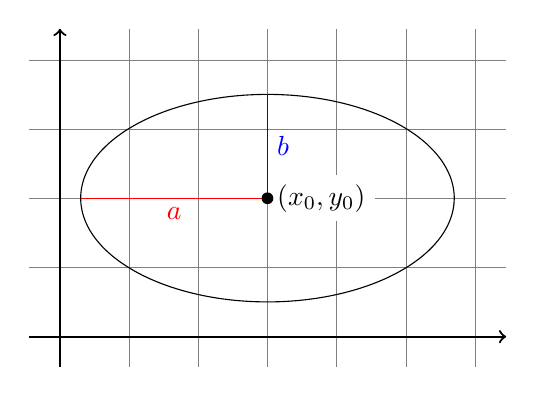
\begin{tikzpicture}[x=0.75pt,y=0.75pt,yscale=-1,xscale=1]
            %coordinatum system
            \foreach \i in {0, ..., 6} {
                \draw [very thin,gray] (\i * 33.33, -15) -- (\i * 33.33, 148);
            }
            \foreach \i in {0, ..., 4} {
                \draw [very thin,gray] (-15 ,\i * 33.33) -- (215 ,\i * 33.33);
            }
            \draw[thick, <-] (0, -15) -- (0, 148);
            \draw[thick, ->] (-15, 133.33) -- (215, 133.33);
            %
            %Ellipse
            \draw plot [smooth, samples = 100, domain = 0:500] ({90 * cos(\x) + 100}, {50 * sin(\x) + 66.6});
            %a
            \draw [red] (100, 66.66) -- (55, 66.66) node[anchor = north, red] {$a$} -- (10, 66.66);
            %b
            \draw [blue] (100, 66.66) -- (100, 41.66) node[anchor = west, blue] {$b$} -- (100, 16.66);
            %Midpoint
            \draw (100, 66.66) node[right, fill=white] {$(x_0, y_0)$} node[circle, fill, inner sep = 1.5pt]{};
        \end{tikzpicture}\\
    \end{center}
    
    \subsubsection{Zykloide}
    \vspace{0.5em}
    \mathbox{
        \overrightarrow{r}(t) = \binom{rt - a \sin(t)}{r - a \cos(t)}
    }
    \text{Sonderfall Gewöhnliche Zykloide } r = a\\
    \begin{center}
        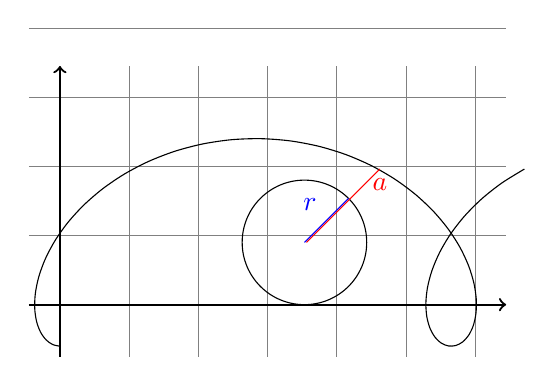
\begin{tikzpicture}[x=0.75pt,y=0.75pt,yscale=1,xscale=1]
            %coordinatum system
            \foreach \i in {0, ..., 6} {
                \draw [very thin,gray] (\i * 33.33, -25) -- (\i * 33.33, 115);
            }
            \foreach \i in {0, ..., 4} {
                \draw [very thin,gray] (-15 ,\i * 33.33) -- (215 ,\i * 33.33);
            }
            \draw[thick, ->] (0, -25) -- (0, 115);
            \draw[thick, ->] (-15, 0) -- (215, 0);
            %
            %Zykloide
            \draw plot [smooth, variable=\x, domain=0:2.75*pi, samples = 50] ({30 * \x - 50 * sin(\x*180/pi)},{30 - 50 * cos(\x*180/pi)});
            %circle
            \draw ({30 * (1.25 * pi)}, 30) circle (30);
            %a
            \draw [red] ({1 + 30 * (1.25 * pi)}, 30) -- ({1 + 30 * (1.25 * pi) - 50 * sin((1.25 * pi)*180/pi)}, {30 - 50 * cos((1.25 * pi)*180/pi)}) node[anchor = north, red] {$a$};
            %radius
            \draw [blue] ({30 * (1.25 * pi)}, 30) -- ({(30 * (1.25 * pi) + 30 * (1.25 * pi) + 30 * 1.414/2)/2}, {(30 + 30 + 30 * 1.414/2)/2}) node[anchor = south east, blue] {$r$} -- ({30 * (1.25 * pi) + 30 * 1.414/2}, {30 + 30 * 1.414/2});
            %
        \end{tikzpicture}\\
    \end{center}

    \vfill \null \columnbreak

    \subsubsection{Epizykloide}
    \vspace{0.5em}
    \mathbox{
        \overrightarrow{r}(t) = \binom{R cos(t) - a cos(\frac{R}{r} t)}{R sin(t) - a sin(\frac{R}{r} t)}
    }
    \text{Sonderfall Kardioide } R = 2r, r = a\\
    \begin{center}
        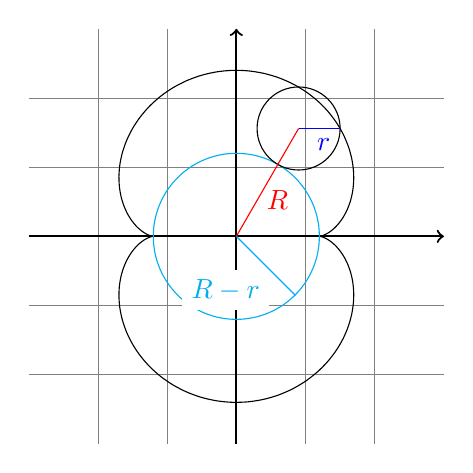
\begin{tikzpicture}[x=0.75pt,y=0.75pt,yscale=1,xscale=1]
            %coordinatum system
            \foreach \i in {-2, ..., 2} {
                \draw [very thin,gray] (\i * 33.33, -100) -- (\i * 33.33, 100);
            }
            \foreach \i in {-2, ..., 2} {
                \draw [very thin,gray] (-100 ,\i * 33.33) -- (100 ,\i * 33.33);
            }
            \draw[thick, ->] (0, -100) -- (0, 100);
            \draw[thick, ->] (-100, 0) -- (100, 0);
            %
            %Epizykloide
            \draw plot [smooth, variable=\x, domain=0:2*pi, samples = 100] ({60 * cos(\x*180/pi) - 20 * cos(60/20 * \x*180/pi)},{60 * sin(\x*180/pi) - 20 * sin(60/20 * \x*180/pi)});
            %big circle
            \draw [cyan] (0, 0) circle (40);
            \draw [cyan] (0, 0) -- (1.424/4 * 45, -1.424/4 * 45) node[anchor = north east, cyan, fill=white] {$R-r$} -- (1.424/2 * 40, -1.424/2 * 40);
            %small circle (t = pi/3)
            \draw ({60 * cos(60)}, {60 * sin(60)}) circle (20);
            %R
            \draw [red] (0, 0) -- ({20 * cos(60)}, {20 * sin(60)}) node[anchor = west, red] {$R$} -- ({60 * cos(60)}, {60 * sin(60)});
            %r
            \draw [blue] ({60 * cos(60)}, {60 * sin(60)}) -- ({60 * cos(60) - 20 * cos(60/20 * 60)},{60 * sin(60) - 20 * sin(60/20 * 60)}) node[anchor = north east, blue] {$r$};
            %
        \end{tikzpicture}\\
    \end{center}

    \subsubsection{Hypozykloide}
    \vspace{0.5em}
    \mathbox{
        \overrightarrow{r}(t) = \binom{R cos(t) + a cos(\frac{R}{r} t)}{R sin(t) - a sin(\frac{R}{r} t)}
    }
    \begin{center}
        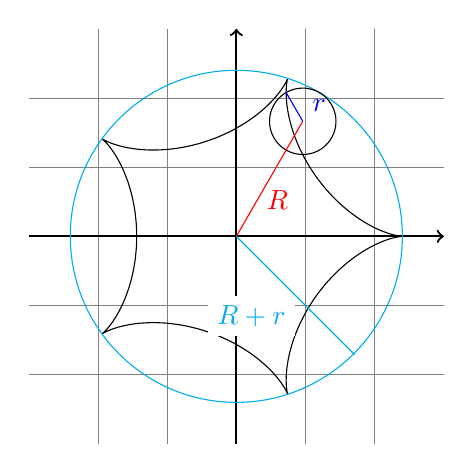
\begin{tikzpicture}[x=0.75pt,y=0.75pt,yscale=1,xscale=1]
            %coordinatum system
            \foreach \i in {-2, ..., 2} {
                \draw [very thin,gray] (\i * 33.33, -100) -- (\i * 33.33, 100);
            }
            \foreach \i in {-2, ..., 2} {
                \draw [very thin,gray] (-100 ,\i * 33.33) -- (100 ,\i * 33.33);
            }
            \draw[thick, ->] (0, -100) -- (0, 100);
            \draw[thick, ->] (-100, 0) -- (100, 0);
            %
            %Hypozykloide
            \draw plot [smooth, variable=\x, domain=0:2*pi, samples = 100] ({64 * cos(\x*180/pi) + 16 * cos(64/16 * \x*180/pi)},{64 * sin(\x*180/pi) - 16 * sin(64/16 * \x*180/pi)});
            %big circle
            \draw [cyan] (0, 0) circle (80);
            \draw [cyan] (0, 0) -- (1.424/4 * 80, -1.424/4 * 80) node[anchor = north east, cyan, fill=white] {$R+r$} -- (1.424/2 * 80, -1.424/2 * 80);
            %small circle (T = pi/3)
            \draw ({64 * cos(60)}, {64 * sin(60)}) circle (16);
            %R
            \draw [red] (0, 0) -- ({20 * cos(60)}, {20 * sin(60)}) node[anchor = west, red] {$R$} -- ({64 * cos(60)}, {64 * sin(60)});
            %r
            \draw [blue] ({64 * cos(60)}, {64 * sin(60)}) node[anchor = south west, blue] {$r$} -- ({64 * cos(60) + 16 * cos(64/16 * 60)},{64 * sin(60) - 16 * sin(64/16 * 60)});
            %
        \end{tikzpicture}\\
    \end{center}

    \subsubsection{Lissajous-Figuren}
    \vspace{0.5em}
    \mathbox{
        \overrightarrow{r}(t) = \binom{a_1 sin(\omega_1 t + \varphi_1)}{a_2 sin(\omega_2 t + \varphi_2)}
    }
        \vfill \null \columnbreak
        \subsection{Häufige Funktionsgraphen}
    \centerline{
        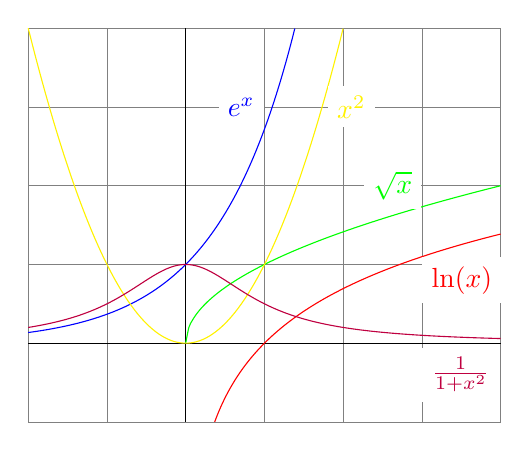
\begin{tikzpicture}
            \draw [help lines] (-2,-1) grid [step=1] (4,4);
            \draw (-2,0) -- (4,0);
            \draw (0,-1) -- (0,4);
            \draw [color = red] plot [smooth, samples = 100, domain = 0.368:4] (\x, {ln(\x)});
                \draw (3, 0.8) node[right, red, fill=white] {$\ln(x)$};
            \draw [color = blue] plot [smooth, samples = 100, domain = -2:1.386] (\x, {e^\x});
                \draw (1,3) node[left, blue, fill=white] {$e^x$};
            \draw [color = green] plot [smooth, samples = 100, domain = 0:4] (\x, {sqrt(\x)});
                \draw (3,2) node[left, green, fill=white] {$\sqrt{x}$};
            \draw [color = yellow] plot [smooth, samples = 100, domain = -2:2] (\x, {(\x)^2});
                \draw (1.8, 3) node[right, yellow, fill=white] {$x^2$};
            \draw [color = purple] plot [smooth, samples = 100, domain = -2:4] (\x, {1/(1+(\x)^2)});
                \draw (3,-0.4
                ) node[right, purple, fill=white] {$\frac{1}{1+x^2}$};
        \end{tikzpicture}
    }
\end{document}